\documentclass[12pt]{article}
\usepackage{listings}
\usepackage{graphicx}
\usepackage{hyperref}

\lstset{
language=Ruby,                  % choose the language of the code
basicstyle=\footnotesize,       % the size of the fonts that are used for the code
numbers=left,                   % where to put the line-numbers
numberstyle=\footnotesize,      % the size of the fonts that are used for the line-numbers
numbersep=5pt,                  % how far the line-numbers are from the code
showspaces=false,               % show spaces adding particular underscores
showstringspaces=false,         % underline spaces within strings
showtabs=false,                 % show tabs within strings adding particular underscores
frame=single,	                  % adds a frame around the code
tabsize=2,	                    % sets default tabsize to 2 spaces
captionpos=b,                   % sets the caption-position to bottom
breaklines=true,                % sets automatic line breaking
breakatwhitespace=false,        % sets if automatic breaks should only happen at whitespace
}

\title{INFO 4300: HW IV} 
\author{Jason Marcell} 
\date{November 7th, 2010}

\begin{document} 
\maketitle 
\newpage
\section{Introduction} % (fold)
\label{sec:introduction}
The purpose of this assignment was to implement the K-Means Clustering Algorithm and perform the algorithm on a corpus of 90 documents in order to observe the effects of varied seed documents and varied number of clusters.
% section introduction (end)

\section{Experiments} % (fold)
\label{sec:experiments}

The first experiment was to run the algorithm on the 90-document corpus with a bisection (i.e. $k = 2$). Seed documents were chosen at random for each run and residual sum of squares was computed for each run of the algorithm. Below are the results of running the algorithm 100 times. Figure 1. shows a histogram of RSS values by frequency. Table 1. shows the statistics for the same run.

\begin{figure}[h!]
  \centering
  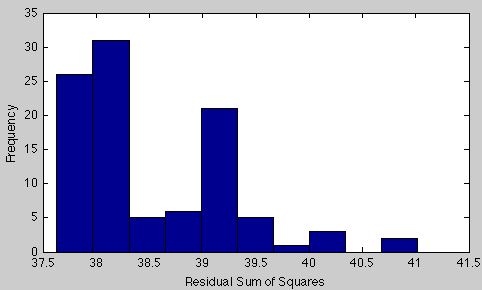
\includegraphics[scale=0.6]{histogram.png}
  \caption{Histogram for Residual Sum of Squares for Bisecting K-Means}
\end{figure}

\begin{table}[h!]
  \centering
  \begin{tabular}{r|l}
    mean      &38.5143\\
    median    &38.2318\\
    mode      &38.1501\\
    std. dev. &0.7458
  \end{tabular}
  \caption{Statistics for Residual Sum of Squares for Bisecting K-Means}
\end{table}

\newpage
The next experiment was to run the K-Means algorithm, varying the value of k. Below, in Figure 2., we see the values of RSS decreasing with increased k-value. There is a noticeable elbow around the value $k = 6$.
\begin{figure}[h!]
  \centering
  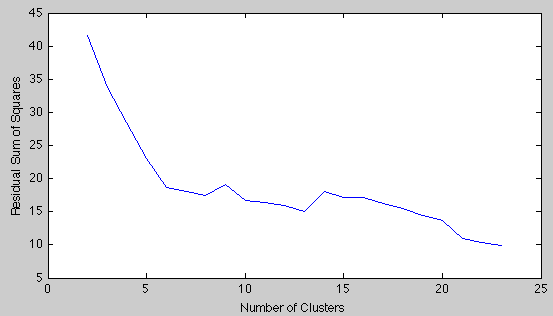
\includegraphics[scale=0.6]{plot.png}
  \caption{RSS Values of K-Means for Various Values of K}
\end{figure}

Finally, we observe multiple trials (3) for a few select values of k (2, 3, 5, 10 and 15). The major observations from this experiment are that the RSS is decreasing and that the implementation of the algorithm seems stable (the RSS  values for a given k-value do not vary wildly, but are instead tightly-clustered with low standard deviation).

\begin{table}[h!]
  \centering
  \begin{tabular}{l|l|l|l}
    K &Trial 1 &Trial 2 &Trial 3\\
    \hline
    2 &38.0832979610152 &38.1501247211226 &38.1501247211226\\
    3 &32.4422541652054 &32.7308133672365 &31.8585706358035\\
    5 &25.3651463086159 &26.1058894419931 &24.0089613268461\\
    10 &16.0332337390105 &16.5255622335598 &16.4953835016395\\
    15 &14.4289801639378 &13.1821955003854 &14.3464196487286\\
  \end{tabular}
  \caption{Trials of K-Means for Various Values of K}
\end{table}

\newpage
\begin{table}[h!]
  \centering
  \begin{tabular}{r|ll}
    topic     &document   &snippet\\
    \hline
    biology   &file14.txt &Insects sense danger on mammals breath\\
    space     &file03.txt &NASA's First Robotic Crew Member to Tweet\\
    internet  &file25.txt &Will Facebook face Apple in trying
  \end{tabular}
  \caption{Topic Labels for K=3 Clustering}
\end{table}

Despite the elbow in Figure 2., indicating that the ideal value for $k$ is about 6, my own experiment and attempts at labeling the clusters seem to indicate that there are roughly three clusters: biology, space, and internet technology.

I started by computing the document that is closest to the centroids for each cluster in a $k = 6$ clustering. I then visually inspected the representative documents for each cluster and attempted to come up with a keyword or two that would describe each cluster. After attempting this for $k = 6$, I noticed that there appeared to be only 3 clearly distinguishable clusters, so I repeated the experiment with $k = 3$, this time modifying my code to output some snippets of the documents in each cluster to confirm my hypothesis.

% section experiments (end)
\newpage
\section{Instructions for Running} % (fold)
\label{sec:instructions_for_running}
The program may be run by typing \texttt{ruby main.rb} from the root of the project folder. 

All software was tested on \texttt{snoopy.cs.cornell.edu}. A local version of \texttt{ruby 1.8.8dev (2010-10-30) [i686-linux]} was installed at \newline
\texttt{/home/jrm425/usr/local/bin/ruby}. A local version of \texttt{rubygems 1.3.7} was installed at \texttt{/home/jrm425/usr/local/bin/gem}.
% section instructions_for_running (end)

\section{References} % (fold)
\label{sec:references}
\begin{itemize}
  \item Formulas were used as per definition from the class website: \url{http://www.infosci.cornell.edu/Courses/info4300/2010fa/index.html}
  \item I collaborated with Karan Kurani for this project.
\end{itemize}
% section references (end)
\end{document}